In this section, we present an approach to uncertainty quantification that forms
the core of the proposed framework. The approach belongs to the class of
stochastic collocation techniques \cite{xiu2010}. The major distinctive feature
of stochastic collocation is the usage of interpolation as a means of
uncertainty quantification, which should be contrasted with other techniques
such as polynomial chaos expansions relying on regression. The algorithm that we
use is based on adaptive sparse-grid interpolation, and it was developed in
\cite{klimke2006} and \cite{ma2009}.

Let $f$ be an uncertain quantity that we are interested in studying. The
quantity is viewed as a vector of $\nout$ deterministic functions each of which
is parametrized by the same set of $\nin$ random variables. Each function
belongs to $\continuous([0, 1]^\nin)$, the space of continuous functions defined
on the unit hypercube $[0, 1]^\nin$. Thus, we have
\[
  f: [0, 1]^\nin \to \real^\nout \subset \continuous([0, 1]^\nin).
\]
Note that the domain $[0, 1]^\nin$ is not a restriction.

The function is assumed to be computationally intensive and impractical for
extensive evaluation, which is needed for Monte Carlo sampling. For example, the
concise notation $f$ might expand into a full-system simulation, including
scheduling and power-temperature analysis, which is the case in this work.

In order to make the problem computationally tractable, a light representation
of $f$ is constructed and studied instead of $f$. The surrogate is based on
interpolation: $f$ is evaluated at a small number of points or nodes, and any
other values of $f$ are reconstructed on demand using a set of basis functions
mediating between the obtained values of $f$.

In what follows, we shall gradually construct an efficient interpolant for $f$.
\emph{Efficiency}, in this context, refers to the number of nodes required to
achieve a certain accuracy level.

\subsection{Tensor Product}
In one dimension ($\nin = 1$), $\f$ is approximated by virtue of the following
interpolation formula:
\begin{equation} \elab{tensor-1d}
  \tensor{i}(\f) := \sum_{j \in \index_i} \f(\x_{ij}) \, \e_{ij}.
\end{equation}
The superscript $i \in \natural$ signifies the level of interpolation; $\X_i =
\{ \x_{ij} \}_{j \in \index_i} \subset [0, 1]$ are the collocation nodes; $\E_i
= \{ \e_{ij} \}_{j \in \index_i} \subset \continuous([0, 1])$ are the basis
functions; and $\index_i = \{ j - 1 \}_{j = 1}^{n_i}$ is an index set
enumerating (starting from zero) the nodes and functions that belong to level
$i$. We shall refer to the subscript $j \in \index_i$ as the order of a node or
function. The choice of the collocation nodes and basis functions is an
important concern, and it will be discussed thoroughly later on.

In multiple dimensions ($\nin > 1$), $\f$ is approximated by the tensor product
of $\nin$ one-dimensional interpolants:
\begin{equation} \elab{tensor}
  \tensor{\vi}(\f) := \left( \bigotimes_{k = 1}^\nin \tensor{i_k} \right)(\f) = \sum_{\vj \in \index_\vi} \f(\vx_{\vi\vj}) \, \e_{\vi\vj}
\end{equation}
where $\vi = (i_k)_{k = 1}^\nin \in \natural^\nin$ and $\vj = (j_k)_{k = 1}^\nin
\in \natural^\nin$ are multi-indices specifying levels and orders, respectively,
for each of the dimensions, and $\index_\vi := \index_{i_1} \times \cdots \times
\index_{i_\nin}$ is a multi-index set obtained by computing the tensor product
of one-dimensional index sets. In the above formula,
\begin{align}
  \X_\vi &= \X_{i_1} \times \cdots \times \X_{i_\nin} \elab{collocation-nodes} \\
         &= \left\{ \vx_{\vi\vj} = (\x_{i_k j_k})_{k = 1}^\nin \right\}_{\vj \in \index_\vi} \subset [0, 1]^\nin \nonumber
\end{align}
and
\begin{equation} \elab{basis-functions}
  \E_\vi = \bigotimes_{k = 1}^\nin \E_{i_k}
         = \left\{ \e_{\vi\vj} = \bigotimes_{k = 1}^\nin \e_{i_k j_k} \right\}_{\vj \in \index_\vi} \subset \continuous([0, 1]^\nin)
\end{equation}
are the collocation nodes and basis functions, respectively, corresponding to
multi-index $\vi$. In \eref{basis-functions}, for any $\vx \in [0, 1]^\nin$,
\begin{equation} \elab{basis-function}
  \e_{\vi\vj}(\vx) = \left( \bigotimes_{k = 1}^\nin \e_{i_k j_k} \right)(\vx) := \prod_{k = 1}^\nin \e_{i_k j_k}(\x_k).
\end{equation}
Lastly, the cardinality of $\index_\vi$ is as follows:
\begin{equation} \elab{tensor-cardinality}
  \n_\vi = \prod_{k = 1}^\nin \n_{i_k}.
\end{equation}
Equation \eref{tensor-cardinality} elucidates the prohibited expense of the
tensor-product construction shown in \eref{tensor} for multidimensional
problems: the number of nodes grows exponentially as $\nin$ increases. However,
\eref{tensor} serves well as a building block for more efficient algorithms,
which we discuss next.

\begin{remark}
Each dimension can have its own rule defining the distribution of collocation
node with respect to each level. Similarly, the basis functions of one dimension
can differ from the basis functions of another. For simplicity and clarity of
presentation, this aspect is not covered in this paper.
\end{remark}


\subsection{Smolyak Algorithm}
One of the central algorithms in the field of high-dimensional integration and
interpolation is the Smolyak algorithm \cite{smolyak1963}. The technique was
developed in the 1960s by Sergey Smolyak, and its impact is comparable to the
one of Monte Carlo sampling. Intuitively speaking, the algorithm takes a number
of small tensor-product structures and composes them in such a way that the
resulting grid has a drastically reduced number of nodes while preserving the
approximating power of the full tensor-product construction for the classes of
functions that one is typically interested in integrating or interpolating
\cite{klimke2006}.

The Smolyak interpolant for $\f$ is as follows:
\begin{equation} \elab{smolyak}
  \smolyak{l}(\f) := \sum_{l - \nin + 1 \leq |\vi|_1 \leq l} (-1)^{l - |\vi|_1} \, {\nin - 1 \choose l - |\vi|_1} \, \tensor{\vi}(\f)
\end{equation}
where $l \in \natural$ is the level of Smolyak's interpolation, and $|\vi|_1 :=
i_1 + \dots + i_\nin$. We see that the algorithm is indeed just a peculiar
composition of cherry-picked tensor products. However, the formula has an
implication of paramount importance: the quantity of interest needs to be
evaluated only at the nodes of the sparse grid underpinning \eref{smolyak}:
\begin{equation} \elab{smolyak-grid}
  \Y^l = \bigcup_{l - \nin + 1 \leq |\vi|_1 \leq l} \X^\vi.
\end{equation}
The cardinality of the above set does not have a general closed-form formula;
however, it can be several orders of magnitude smaller than the one of the full
tensor product given in \eref{tensor-cardinality}, which depends on the
dimensionality of the problem at hand and the one-dimensional rules utilized.

A better intuition about the properties of Smolyak's construction can be
obtained by rewriting \eref{smolyak} in an incremental form. To this end, let
$\Delta\tensor{-1}(\f) := 0$,
\begin{align}
  & \Delta\tensor{i}(\f) := (\tensor{i} - \tensor{i - 1})(\f), \text{ and} \elab{tensor-delta-1d} \\
  & \Delta\tensor{\vi}(\f) := (\Delta\tensor{i_1} \otimes \cdots \otimes
  \Delta\tensor{i_\nin})(\f). \nonumber
\end{align}
Then, \eref{smolyak} is identical to
\begin{equation} \elab{smolyak-incremental}
  \smolyak{l}(\f) = \sum_{|\vi|_1 \leq l} \Delta\tensor{\vi}(\f) = \smolyak{l - 1}(\f) + \sum_{|\vi|_1 = l} \Delta\tensor{\vi}(\f)
\end{equation}
where $\smolyak{-1}(\f) := 0$. It can be seen that a Smolyak interpolant can be
refined efficiently: the work done to attain one accuracy level can be entirely
recycled to go one level up.

The sparsity and incremental refinement of Smolyak's approach, which are shown
in \eref{smolyak-grid} and \eref{smolyak-incremental}, respectively, are
remarkable properties \perse, but they can be taken even further. To this end,
let $\Delta\X^{-1} := \emptyset$,
\begin{align*}
  & \Delta\X^i := \X^i \setminus \X^{i - 1}, \text{ and} \\
  & \Delta\X^\vi := \Delta\X^{i_1} \times \cdots \times \Delta\X^{i_\nin}.
\end{align*}
Then, \eref{smolyak-grid} can be rewritten as
\begin{equation} \elab{smolyak-grid-incremental}
  \Y^l = \bigcup_{|\vi|_1 \leq l} \Delta\X^\vi = \Y^{l - 1} \cup \bigcup_{|\vi|_1 = l} \Delta\X^\vi,
\end{equation}
which is analogous to \eref{smolyak-incremental}. It can be seen now that it is
beneficial for refinement to have $\X^{i - 1}$ be entirely included in $\X^i$
since, in that case, the cardinality of $\Y^l \setminus \Y^{l - 1} =
\bigcup_{|\vi|_1 = l} \Delta\X^\vi$ derived from \eref{smolyak-grid-incremental}
decreases. In words, the values of $\f$ obtained on lower levels can be reused
to attain higher levels if the grid grows without abandoning its previous
structure. With this in mind, the rule used for generating successive sets of
points $\{ \X^i \}_{i \in \natural}$ should be chosen to be nested, that is, in
such a way that $\X^i$ contains all nodes of $\X^{i - 1}$. By doing so, the
incremental refinement really starts to shine.

Lastly, we need to impose one additional property in order to rewrite
\eref{smolyak-incremental} in a hierarchical form. Namely, we require the
interpolants of higher levels to represent exactly the interpolants of lower
levels. In one dimension, it means that
\begin{equation} \elab{tensor-exactness}
  \tensor{i - 1}(\f) = \tensor{i}(\tensor{i - 1}(\f)).
\end{equation}
The condition in \eref{tensor-exactness} can be satisfied by an appropriate
choice of collocation nodes and basis functions, which will be discussed later.
If \eref{tensor-exactness} holds, using \eref{tensor-1d} and
\eref{tensor-delta-1d},
\[
  \Delta\tensor{i}(\f) = \sum_{j \in \Delta\index(i)} \left( \f(\x^i_j) - \tensor{i - 1}(\f)(\x^i_j) \right) \, \e^i_j
\]
where $\Delta\index(i) := \{ j \in \index(i): \x^i_j \in \Delta\X^i \}$. The
above sum is over $\Delta\X^i$ due to the fact that the difference in the
parentheses is zero whenever $\x^i_j \in \X^{i - 1}$ since $\X^{i - 1} \subset
\X^i$. In multiple dimensions, using the Smolyak formula, we have
\begin{equation} \elab{tensor-delta}
  \Delta\tensor{\vi}(\f) = \sum_{\vj \in \Delta\index(\vi)} \left( \f(\vx^\vi_\vj) - \smolyak{|\vi|_1 - 1}(\f)(\vx^\vi_\vj) \right) \, \e^\vi_\vj
\end{equation}
where $\Delta\index(\vi) := \{ \vj \in \index(\vi): \vx^\vi_\vj \in \Delta\X^\vi
\}$. The delta
\begin{equation} \elab{surplus}
  \surplus(\vx^\vi_\vj) := \f(\vx^\vi_\vj) - \smolyak{|\vi|_1 - 1}(\f)(\vx^\vi_\vj)
\end{equation}
is called a hierarchical surplus. When increasing the interpolation level, this
surplus is nothing but the difference between the actual value of $\f$ at a new
node and the approximation of this value computed by the interpolant constructed
so far.

The final formula for nonadaptive hierarchical interpolation is obtained by
substituting \eref{tensor-delta} into \eref{smolyak-incremental}:
\begin{equation} \elab{smolyak-hierarchical}
  \smolyak{l}(\f) = \smolyak{l-1}(\f) + \sum_{|\vi|_1 = l} \, \sum_{\vj \in \Delta\index(\vi)} \surplus(\vx^\vi_\vj) \, \e^\vi_\vj
\end{equation}
where $\surplus(\vx^\vi_\vj)$ is computed according to \eref{surplus}.


\subsection{Grid Nodes}
We use the open Newton--Cotes interpolation grid \cite{klimke2006}.

\subsection{Basis Functions}
We use the linear hat functions as the basis functions \cite{klimke2006}.

In this section, we present the interpolation algorithm that forms the core of
the proposed framework for probabilistic analysis of electronic systems. The
algorithm is based on the work in \cite{jakeman2012, klimke2006, ma2009}, and it
features a sparse-grid structure, hierarchical construction, and hybrid
adaptivity. The benefits of these features are interconnected and can be
summarized as follows: the ability to mitigate the curse of dimensionality and,
thereby, tackle multidimensional problems; the ability to perform gradual
refinement of the approximation with a natural error control; and the ability to
make the refinement fine-grained and, hence, gain further efficiency.

Let $\f$ be a function that we would like to approximate. The function is
assumed to be in $\continuous([0, 1]^\nin)$, the space of continuous functions
in the unit hypercube $[0, 1]^\nin$. The assumption is a formality, and the
interpolation algorithm discussed in \sref{implementation} can be applied to
functions with finite discontinuities as well, which is actually the case in the
example given in \fref{motivation}. Furthermore, the domain $[0, 1]^\nin$ is
merely standardization rather than a restriction.

In what follows, we shall gradually construct an efficient interpolant for $\f$.
Efficiency here refers to the number of collocation nodes required to achieve a
certain accuracy level.

\subsection{Tensor Product} \slab{tensor-product}
In one dimension ($\nin = 1$), $\f$ is approximated by virtue of the following
interpolation formula:
\begin{equation} \elab{tensor-1d}
  \tensor{i}(\f) := \sum_{j \in \index_i} \f(\x_{ij}) \, \e_{ij}.
\end{equation}
The superscript $i \in \natural$ signifies the level of interpolation; $\X_i =
\{ \x_{ij} \}_{j \in \index_i} \subset [0, 1]$ are the collocation nodes; $\E_i
= \{ \e_{ij} \}_{j \in \index_i} \subset \continuous([0, 1])$ are the basis
functions; and $\index_i = \{ j - 1 \}_{j = 1}^{n_i}$ is an index set
enumerating (starting from zero) the nodes and functions that belong to level
$i$. We shall refer to the subscript $j \in \index_i$ as the order of a node or
function. The choice of the collocation nodes and basis functions is an
important concern, and it will be discussed thoroughly later on.

In multiple dimensions ($\nin > 1$), $\f$ is approximated by the tensor product
of $\nin$ one-dimensional interpolants:
\begin{equation} \elab{tensor}
  \tensor{\vi}(\f) := \left( \bigotimes_{k = 1}^\nin \tensor{i_k} \right)(\f) = \sum_{\vj \in \index_\vi} \f(\vx_{\vi\vj}) \, \e_{\vi\vj}
\end{equation}
where $\vi = (i_k)_{k = 1}^\nin \in \natural^\nin$ and $\vj = (j_k)_{k = 1}^\nin
\in \natural^\nin$ are multi-indices specifying levels and orders, respectively,
for each of the dimensions, and $\index_\vi := \index_{i_1} \times \cdots \times
\index_{i_\nin}$ is a multi-index set obtained by computing the tensor product
of one-dimensional index sets. In the above formula,
\begin{align}
  \X_\vi &= \X_{i_1} \times \cdots \times \X_{i_\nin} \elab{collocation-nodes} \\
         &= \left\{ \vx_{\vi\vj} = (\x_{i_k j_k})_{k = 1}^\nin \right\}_{\vj \in \index_\vi} \subset [0, 1]^\nin \nonumber
\end{align}
and
\begin{equation} \elab{basis-functions}
  \E_\vi = \bigotimes_{k = 1}^\nin \E_{i_k}
         = \left\{ \e_{\vi\vj} = \bigotimes_{k = 1}^\nin \e_{i_k j_k} \right\}_{\vj \in \index_\vi} \subset \continuous([0, 1]^\nin)
\end{equation}
are the collocation nodes and basis functions, respectively, corresponding to
multi-index $\vi$. In \eref{basis-functions}, for any $\vx \in [0, 1]^\nin$,
\begin{equation} \elab{basis-function}
  \e_{\vi\vj}(\vx) = \left( \bigotimes_{k = 1}^\nin \e_{i_k j_k} \right)(\vx) := \prod_{k = 1}^\nin \e_{i_k j_k}(\x_k).
\end{equation}
Lastly, the cardinality of $\index_\vi$ is as follows:
\begin{equation} \elab{tensor-cardinality}
  \n_\vi = \prod_{k = 1}^\nin \n_{i_k}.
\end{equation}
Equation \eref{tensor-cardinality} elucidates the prohibited expense of the
tensor-product construction shown in \eref{tensor} for multidimensional
problems: the number of nodes grows exponentially as $\nin$ increases. However,
\eref{tensor} serves well as a building block for more efficient algorithms,
which we discuss next.

\begin{remark}
Each dimension can have its own rule defining the distribution of collocation
node with respect to each level. Similarly, the basis functions of one dimension
can differ from the basis functions of another. For simplicity and clarity of
presentation, this aspect is not covered in this paper.
\end{remark}


\subsection{Smolyak Algorithm} \slab{smolyak-algorithm}
One of the central algorithms in the field of high-dimensional integration and
interpolation is the Smolyak algorithm \cite{smolyak1963}. The technique was
developed in the 1960s by Sergey Smolyak, and its impact is comparable to the
one of Monte Carlo sampling. Intuitively speaking, the algorithm takes a number
of small tensor-product structures and composes them in such a way that the
resulting grid has a drastically reduced number of nodes while preserving the
approximating power of the full tensor-product construction for the classes of
functions that one is typically interested in integrating or interpolating
\cite{klimke2006}.

The Smolyak interpolant for $\f$ is as follows:
\begin{equation} \elab{smolyak}
  \smolyak{l}(\f) := \sum_{l - \nin + 1 \leq |\vi|_1 \leq l} (-1)^{l - |\vi|_1} \, {\nin - 1 \choose l - |\vi|_1} \, \tensor{\vi}(\f)
\end{equation}
where $l \in \natural$ is the level of Smolyak's interpolation, and $|\vi|_1 :=
i_1 + \dots + i_\nin$. We see that the algorithm is indeed just a peculiar
composition of cherry-picked tensor products. However, the formula has an
implication of paramount importance: the quantity of interest needs to be
evaluated only at the nodes of the sparse grid underpinning \eref{smolyak}:
\begin{equation} \elab{smolyak-grid}
  \Y^l = \bigcup_{l - \nin + 1 \leq |\vi|_1 \leq l} \X^\vi.
\end{equation}
The cardinality of the above set does not have a general closed-form formula;
however, it can be several orders of magnitude smaller than the one of the full
tensor product given in \eref{tensor-cardinality}, which depends on the
dimensionality of the problem at hand and the one-dimensional rules utilized.

A better intuition about the properties of Smolyak's construction can be
obtained by rewriting \eref{smolyak} in an incremental form. To this end, let
$\Delta\tensor{-1}(\f) := 0$,
\begin{align}
  & \Delta\tensor{i}(\f) := (\tensor{i} - \tensor{i - 1})(\f), \text{ and} \elab{tensor-delta-1d} \\
  & \Delta\tensor{\vi}(\f) := (\Delta\tensor{i_1} \otimes \cdots \otimes
  \Delta\tensor{i_\nin})(\f). \nonumber
\end{align}
Then, \eref{smolyak} is identical to
\begin{equation} \elab{smolyak-incremental}
  \smolyak{l}(\f) = \sum_{|\vi|_1 \leq l} \Delta\tensor{\vi}(\f) = \smolyak{l - 1}(\f) + \sum_{|\vi|_1 = l} \Delta\tensor{\vi}(\f)
\end{equation}
where $\smolyak{-1}(\f) := 0$. It can be seen that a Smolyak interpolant can be
refined efficiently: the work done to attain one accuracy level can be entirely
recycled to go one level up.

The sparsity and incremental refinement of Smolyak's approach, which are shown
in \eref{smolyak-grid} and \eref{smolyak-incremental}, respectively, are
remarkable properties \perse, but they can be taken even further. To this end,
let $\Delta\X^{-1} := \emptyset$,
\begin{align*}
  & \Delta\X^i := \X^i \setminus \X^{i - 1}, \text{ and} \\
  & \Delta\X^\vi := \Delta\X^{i_1} \times \cdots \times \Delta\X^{i_\nin}.
\end{align*}
Then, \eref{smolyak-grid} can be rewritten as
\begin{equation} \elab{smolyak-grid-incremental}
  \Y^l = \bigcup_{|\vi|_1 \leq l} \Delta\X^\vi = \Y^{l - 1} \cup \bigcup_{|\vi|_1 = l} \Delta\X^\vi,
\end{equation}
which is analogous to \eref{smolyak-incremental}. It can be seen now that it is
beneficial for refinement to have $\X^{i - 1}$ be entirely included in $\X^i$
since, in that case, the cardinality of $\Y^l \setminus \Y^{l - 1} =
\bigcup_{|\vi|_1 = l} \Delta\X^\vi$ derived from \eref{smolyak-grid-incremental}
decreases. In words, the values of $\f$ obtained on lower levels can be reused
to attain higher levels if the grid grows without abandoning its previous
structure. With this in mind, the rule used for generating successive sets of
points $\{ \X^i \}_{i \in \natural}$ should be chosen to be nested, that is, in
such a way that $\X^i$ contains all nodes of $\X^{i - 1}$. By doing so, the
incremental refinement really starts to shine.

Lastly, we need to impose one additional property in order to rewrite
\eref{smolyak-incremental} in a hierarchical form. Namely, we require the
interpolants of higher levels to represent exactly the interpolants of lower
levels. In one dimension, it means that
\begin{equation} \elab{tensor-exactness}
  \tensor{i - 1}(\f) = \tensor{i}(\tensor{i - 1}(\f)).
\end{equation}
The condition in \eref{tensor-exactness} can be satisfied by an appropriate
choice of collocation nodes and basis functions, which will be discussed later.
If \eref{tensor-exactness} holds, using \eref{tensor-1d} and
\eref{tensor-delta-1d},
\[
  \Delta\tensor{i}(\f) = \sum_{j \in \Delta\index(i)} \left( \f(\x^i_j) - \tensor{i - 1}(\f)(\x^i_j) \right) \, \e^i_j
\]
where $\Delta\index(i) := \{ j \in \index(i): \x^i_j \in \Delta\X^i \}$. The
above sum is over $\Delta\X^i$ due to the fact that the difference in the
parentheses is zero whenever $\x^i_j \in \X^{i - 1}$ since $\X^{i - 1} \subset
\X^i$. In multiple dimensions, using the Smolyak formula, we have
\begin{equation} \elab{tensor-delta}
  \Delta\tensor{\vi}(\f) = \sum_{\vj \in \Delta\index(\vi)} \left( \f(\vx^\vi_\vj) - \smolyak{|\vi|_1 - 1}(\f)(\vx^\vi_\vj) \right) \, \e^\vi_\vj
\end{equation}
where $\Delta\index(\vi) := \{ \vj \in \index(\vi): \vx^\vi_\vj \in \Delta\X^\vi
\}$. The delta
\begin{equation} \elab{surplus}
  \surplus(\vx^\vi_\vj) := \f(\vx^\vi_\vj) - \smolyak{|\vi|_1 - 1}(\f)(\vx^\vi_\vj)
\end{equation}
is called a hierarchical surplus. When increasing the interpolation level, this
surplus is nothing but the difference between the actual value of $\f$ at a new
node and the approximation of this value computed by the interpolant constructed
so far.

The final formula for nonadaptive hierarchical interpolation is obtained by
substituting \eref{tensor-delta} into \eref{smolyak-incremental}:
\begin{equation} \elab{smolyak-hierarchical}
  \smolyak{l}(\f) = \smolyak{l-1}(\f) + \sum_{|\vi|_1 = l} \, \sum_{\vj \in \Delta\index(\vi)} \surplus(\vx^\vi_\vj) \, \e^\vi_\vj
\end{equation}
where $\surplus(\vx^\vi_\vj)$ is computed according to \eref{surplus}.


\subsection{Collocation Nodes} \slab{collocation-nodes}
A sparse grid that is fully nested and well suited for local adaptivity, which
we requested previous, can be constructed using the (one-dimensional)
Newton--Cotes rule \cite{klimke2006, ma2009}. For each level, the rule is merely
a set of equidistant nodes on an interval, which is $[0, 1]$ in our case.

\begin{remark}
Equidistant nodes are known to perform poorly when the interpolating functions
are polynomials (Runge's phenomenon). However, it is not a concern for us as our
basis functions are not exposed to this problem.
\end{remark}

The rule comes in two flavors: closed and open. The only difference between the
two is that the former includes the endpoints, that is, 0 and 1, while the
latter does not. Now, at the end of \sref{smolyak-algorithm}, we postulated that
the assumption in \eref{tensor-exactness} was needed to proceed. The closed rule
satisfies this assumption while the open one violates it close to the boundaries
of the interval. However, as noted in \cite{klimke2006}, the open Newton--Cotes
rule is a viable option since it performs well in practice. We were able to
achieve better results using the open rule, and, therefore, we have decided to
present it in the paper.

\begin{figure}[t]
  \centering
  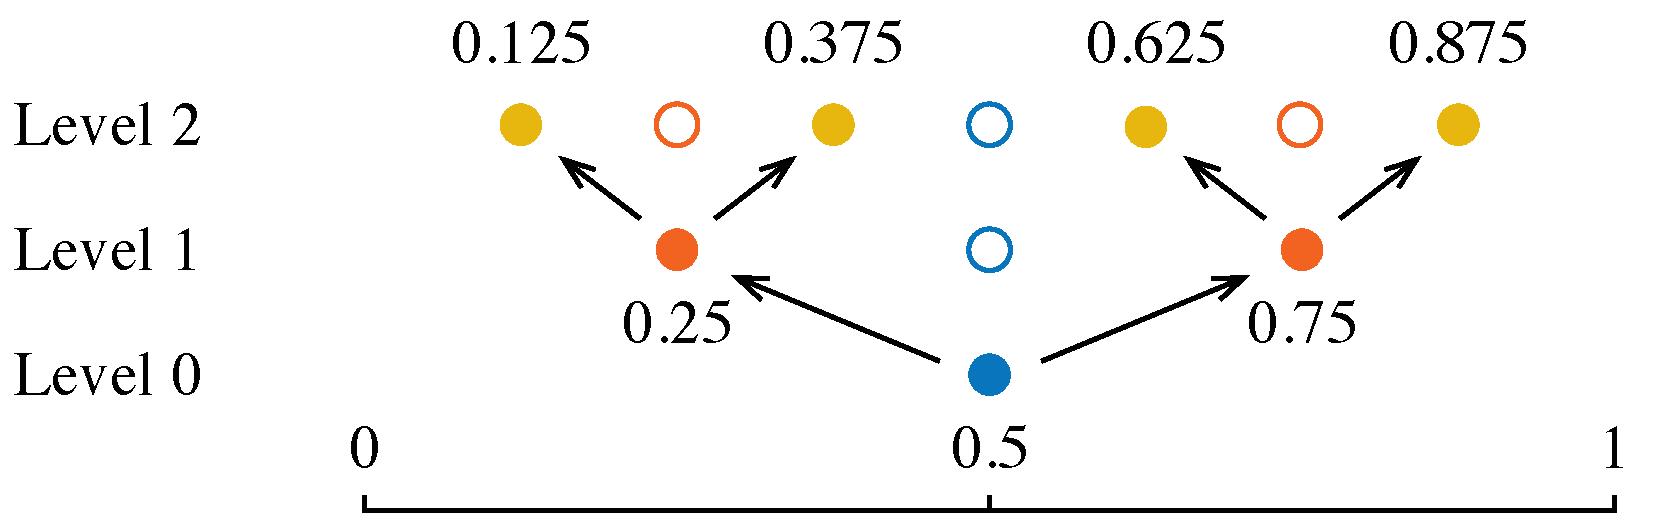
\includegraphics[width=1.0\columnwidth]{include/assets/figures/rule.pdf}
  \caption{
    An illustration of the open Newton--Cotes rule on $[0, 1]$. On each level,
    the dots correspond to the nodes introduced by that particular level, and
    the wholes correspond to the nodes inherited from the previous levels.
  }
  \flab{rule}
\end{figure}

The open Newton--Cotes rule of level $i \in \natural$ is
\begin{equation} \elab{newton-cotes-grid}
  \X_i = \left\{ x_{ij} = \frac{j + 1}{\n_i + 1}: j \in \index_i \right\}
\end{equation}
where $\index_i = \left\{ 0, \dots, \n_i - 1 \right\}$ with $\n_i = 2^{i + 1} -
1$. The first three levels of the rule are depicted in \fref{rule}. It can be
seen that the number of nodes (in one dimension) grows as 1, 3, 7, 15, 31, and
so on, and the rule is fully nested. In multiple dimensions, the nodes are
formed as shown in \eref{collocation-nodes}.

Figure~\ref{fig:rule} also illustrates a refinement procedure suitable for this
grid. The arrows emerging from a node connect the node with its next-level
neighbors. The number of such neighbors is two in one dimension and $2 \nin$ in
general. Formally, for a pair $(\vi, \vj)$, the neighbor pairs are
\[
  \left\{ \Big( (i_1, \dots, i_k + 1, \dots, i_\nin), (j_1, \dots, 2 j_k + c, \dots j_\nin) \Big) \right\}_{k, c}
\]
for $k = 1, \dots, \nin$ and $c \in \{ 0, 2 \}$. Whenever a node is chosen for
refinement, some or all of its neighbors can be added to the interpolant. One
possible strategy is to include all $2 \nin$ neighbors, which is what we shall
do.

\begin{remark}
It is important to note that an arbitrary set of nodes identified by some pairs
$\{ (\vi_k, \vj_k) \}_k$ does not necessarily correspond to a valid
construction. In order to have a valid construction, the multi-indices $\{ \vi_k
\}_k$ should satisfy a so-called admissibility condition \cite{klimke2006}. The
condition is diligently satisfied when the refinement is undertaken level by
level following neighbor connections, which is what we do.
\end{remark}

First of all, looking at \eref{smolyak-hierarchical}, it is not clear what the
interpolation level $\l$ should be in order to achieve a certain accuracy level.
When should we stop?


\subsection{Basis Functions} \slab{basis-functions}
\begin{figure}[t]
  \centering
  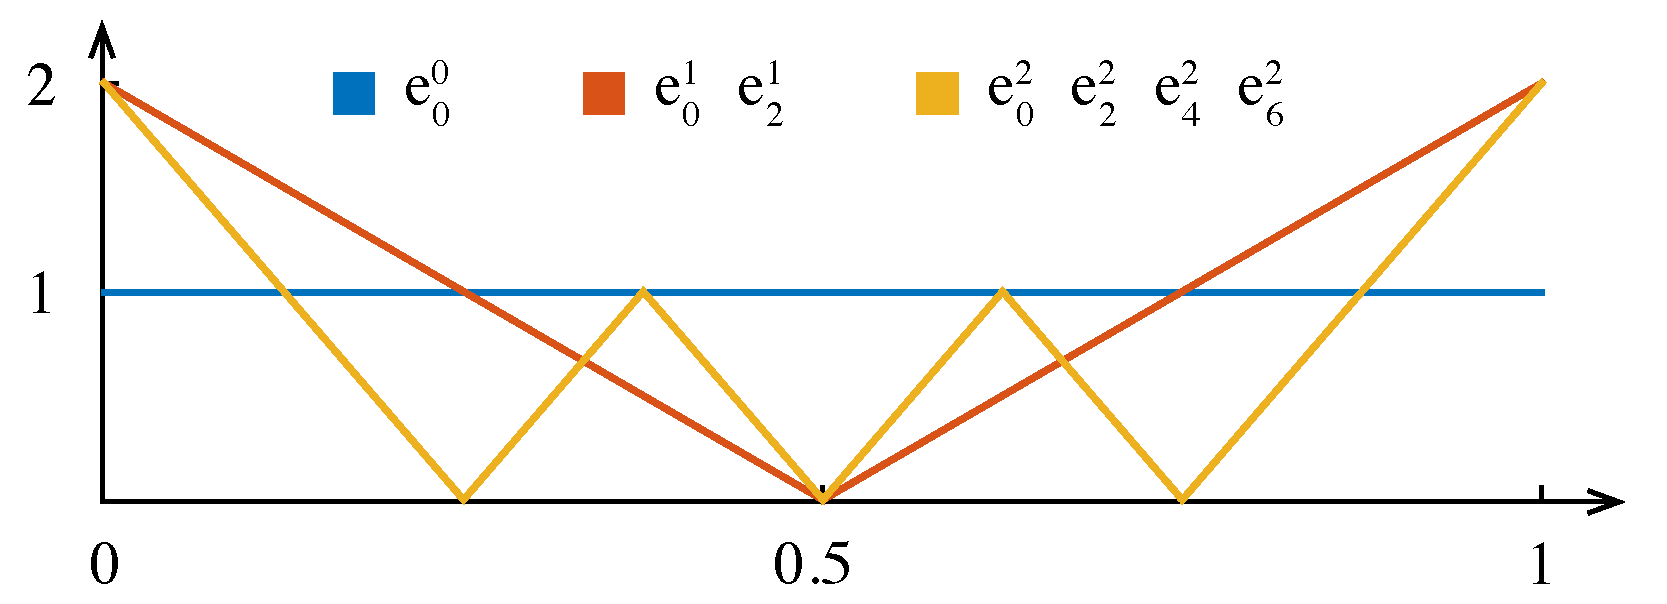
\includegraphics[width=1.0\columnwidth]{include/assets/figures/basis.pdf}
  \vspace{-1.5em}
  \caption{
    The first three levels of the basis described in \sref{basis}.
  }
  \flab{basis}
\end{figure}

The basis functions that go hand in hand with the open Newton--Cotes rule are
the following piecewise linear functions. For $i = 0$ and $j = 0$,
\[
  \e_{00}(\x) = 1.
\]
For $i > 0$ and $j = 0$ (close to the left endpoint),
\[
  \e_{i0}(\x) = \begin{cases}
    2 - \left( \n_i + 1 \right) \x, & \text{if } \x < \frac{2}{\n_i + 1}, \\
    0, & \text{otherwise}.
  \end{cases}
\]
For $i > 0$ and $j = \n_i - 1$ (close to the right endpoint),
\[
  \e_{i(\n_i - 1)}(\x) = \begin{cases}
    \left( \n_i + 1 \right) \x - \n_i + 1, & \text{if } \x > \frac{\n_i - 1}{\n_i + 1}, \\
    0, & \text{otherwise}.
  \end{cases}
\]
In other cases,
\[
  \e_{ij}(\x) = \begin{cases}
    1 - \left( \n_i + 1 \right)|\x - \x_{ij}|, & \text{if } |\x - \x_{ij}| < \frac{1}{\n_i + 1}, \\
    0, & \text{otherwise}.
  \end{cases}
\]
The basis functions corresponding to the first three levels of one-dimensional
interpolation are depicted in \fref{basis}. Note that $\e_{11}$, $\e_{21}$,
$\e_{23}$, and $\e_{25}$ are not depicted as they are not involved in the
hierarchical construction. In multiple dimensions, the basis functions are
formed as shown in \eref{basis-functions}.

Lastly, let us mention the volumes (integrals over the whole domain) of the
basis functions denoted by $\w_{ij}$; they will be needed in the future. Namely,
$\w_{00} = 1$ and, for $i > 0$,
\begin{equation} \elab{volume}
  \w_{ij} := \int_0^1 \e_{ij}(\x) \, \d\x = \begin{cases}
    \frac{2}{\n_i + 1}, & \text{if } j \in \{ 0, \n_i - 1 \}, \\
    \frac{1}{\n_i + 1}, & \text{otherwise}.
  \end{cases}
\end{equation}
In multiple dimensions, the volumes are products of the one-dimensional
components, analogous to \eref{basis-function}.

\begin{remark}
Instead of piecewise linear functions, one can also utilize locally supported
polynomials of higher orders \cite{jakeman2012}. However, we did not observe
much improvement and, therefore, do not discuss this alternative in the paper.
\end{remark}


\subsection{Adaptivity} \slab{adaptivity}
We are ready to discuss adaptivity, and we begin by reiterating briefly out
motivation. Imagine a function that is nearly flat on the first half of $[0, 1]$
and rather irregular on the other. Under these circumstances, it is natural to
expect that, in order to attain the same accuracy, the first half would require
much fewer collocation nodes than the other one; recall the example given in
\fref{motivation}. However, if we followed the construction procedure described
so far, we would not be able to benefit from the peculiar behavior: we would
treat both sides equally and would add all the nodes of each level.

The solution to the above problem is to make the interpolation algorithm
adaptive. First of all, we need to find a way to measure how good our
approximation is at any point in the domain of $\f$. Then, when taking an
interpolation step, instead of bombarding $\f$ with all the nodes that can be
legitimately added to the interpolant at that step, we will only include those
nodes that are located in the regions with poor accuracy as indicated by the
yet-to-be-found accuracy metric. The outlined strategy practically means that
$\Delta\lindex_\l$ and $\Delta\oindex_\vi$ in \eref{smolyak-hierarchical} will
be only subsets of what is possible at step $\l$.

\begin{remark}
It is important to note that, in general, an arbitrary set of nodes does not
correspond to a valid construction. In order to have a valid interpolant, the
corresponding set of level and order indices, $\{ (\vi_k, \vj_k) \}_k$, should
satisfy the so-called admissibility condition \cite{jakeman2012, klimke2006}.
The condition is diligently satisfied in the algorithms presented here.
\end{remark}

Thanks to the hierarchical form obtained in the previous subsection, we already
have a good candidate for the accuracy metric. Recall \eref{surplus}.
Hierarchical surpluses are a natural indicator of the interpolation error: as
noted earlier, they are the difference between the true function and its
approximation at the nodes of the underlying sparse grid. Consequently, after
computing the surpluses corresponding to the nodes of one level, we can recycle
their values in order to decide which of the nodes are to be refined, that is,
which of the nodes of the next level are to be included in the interpolant.

In order to identify ``problematic'' nodes, one can adhere to various
strategies, and ours is as follows. A collocation node $\vx_{\vi\vj}$ is to be
refined if
\begin{equation} \elab{serror}
  \left| \surplus(\vx_{\vi\vj}) \, \w_{\vi\vj} \right| \ge \serror
\end{equation}
where $\surplus(\vx_{\vi\vj})$ and $\w_{\vi\vj}$ are given by \eref{surplus} and
\eref{volume}, respectively, and $\serror$ is a user-defined constant. We refer
to the left-hand side of \eref{serror} as the score of $\vx_{\vi\vj}$ and to
$\serror$ as the score error. The above criterion will be used in our
experiments.

The question now is: How is the refinement of a node undertaken? The refinement
procedure of the Newton--Cotes rule is illustrated in \fref{rule}. The arrows
emerging from a node connect the node with its forward (next-level) neighbors.
The number of such neighbors is two in one dimension and $2 \nin$ in general.
Formally, for a pair $(\vi, \vj)$, the neighbor pairs are
\begin{align}
  \left\{\vphantom{\Big(}\right. \Big( &(i_1, \dots,   i_k + 1, \dots, i_\nin), \elab{neighbors} \\
                                       &(j_1, \dots, 2 j_k + c, \dots, j_\nin) \Big) \left.\vphantom{\Big)} \right\}_{k, c} \nonumber
\end{align}
for $k = 1, \dots, \nin$ and $c \in \{ 0, 2 \}$. Whenever a node is chosen for
refinement, some or all of its neighbors can be added to the interpolant. The
simplest strategy is to include all $2 \nin$ neighbors of each ``problematic''
node, as in \cite{ma2009}.

Equation \eref{serror} gives us local adaptivity. Local adaptivity operates on
the level of individual nodes. However, it is only one of the two types of
adaptivity that we would like to have. The other one is global adaptivity
\cite{klimke2006}. Global adaptivity operates on the level of individual
dimensions. The intuition behind is that, in general, the input variables
manifest themselves (impact $\f$) differently, and the interpolation algorithm
is likely to benefit by prioritizing those variables that the most influential.
An adaptivity strategy that is both local and global is referred to as hybrid,
and this is our goal in this subsection.

Global adaptivity can be attained by revisiting the set of forward neighbors
given in \eref{neighbors}. The set currently contains the neighbors of a node
with respect to all the dimensions.


To summarize, we have obtained an efficient algorithm for adaptive hierarchical
interpolation in multiple dimensions. The main equations are \eref{surplus} and
\eref{smolyak-hierarchical} where $\vx_{\vi\vj}$ and $\e_{\vi\vj}$ are the ones
given in \sref{collocation-nodes} and \sref{basis-functions}, respectively, and
$\Delta\oindex_\vi$ is generally replaced by its subset according to the hybrid
adaptation strategy presented in \sref{adaptivity}. In the next subsection, we
would like to give an algorithmic structure of the technique in order to
streamline its implementation.

\subsection{Implementation} \slab{implementation}
The life cycle of interpolation has roughly two stages: construction and usage.
The construction stage invokes $\f$ at a set of collocation nodes and produces
certain artifacts. The usage stage estimates the values of $\f$ at a set of
arbitrary (likely unseen) points solely by manipulating the artifacts. It can be
seen in \eref{approximation} that an interpolant is entirely characterized by a
set of triplets $\{ (\vi_k, \vj_k, \surplus(\vx_{\vi_k \vj_k}) \}_k$, which is
obtained by following the recursion and ``flattening'' the nested sums in
\eref{approximation}. These triples are the above-mentioned artifacts.

\begin{algorithm}
  \caption{\emph{Construct} an interpolant of a function.}
  \alab{construct}
  \begin{algorithmic}[1]
    \vspace{0.4em}

    \Require{target} \Comment{A function to interpolate}
    \Ensure{surrogate} \Comment{Artifacts of interpolation}

    \vspace{0.4em}

    \Let{surrogate}{New()}

    \For{s = First(); !Check(s); s = Next(s)}
      \Let{s.nodes}{Locate(s.indices)}
      \Let{s.values}{Invoke(target, s.nodes)}
      \Let{s.estimates}{Evaluate(surrogate, s.nodes)}
      \Let{s.surpluses}{Subtract(s.values, s.estimates)}
      \Let{s.scores}{Assess(s.surpluses)}
      \State Append(surrogate, s.indices, s.surpluses)
    \EndFor

    \State \textbf{return} surrogate

    \vspace{0.4em}
  \end{algorithmic}
\end{algorithm}

The conceptual code corresponding to the construction stage is given in
\aref{construct} called \token{Construct}.

\begin{remark}
The purpose of the pseudocodes presented here is to give the big picture of the
interpolation algorithm, not minute implementation details. Since we open-source
our code, all the details can be found and studied at online \cite{sources}.
\end{remark}

The input \token{target} is a function $\f$ to be approximated. The output
\token{surrogate} is a structure containing the artifacts mentioned earlier:
indexing pairs and surpluses; hereafter, the former are referred to as just
indices. The key steps of the \token{Construct} algorithm are as follows.

\begin{compactlist}

\point{Line~4:} Each iteration of the outermost loop corresponds to a level of
Smolyak's interpolation, which is denoted by $l$ in \eref{smolyak-hierarchical}
and by \token{level} in the code. The \token{indices} variable is a working set
containing the indices of the current (in progress) level. The set is initially
populated on line~2 by the indices of level~0, which is just $\{ (\v{0}, \v{0})
\}$ for the Newton--Cotes grid.

\point{Line~5:} \token{grid.ComputeNodes} takes a set of indices and returns the
corresponding (multidimensional) nodes of the underlying sparse grid; see
\sref{collocation-nodes}.

\point{Line~6:} \token{Invoke} exercises the target function at each of the
given nodes and returns the corresponding values. This is a prominent candidate
for parallelization since each collocation node can be evaluated independently
from the rest.

\point{Line~7:} \token{Evaluate} utilizes the interpolant constructed so far in
order to calculate approximations to the true values of the target function
obtained on line~6. The \token{Evaluate} function is \aref{evaluate}, and it
will be discussed separately.

\point{Line~9--10:} \token{Append} ameliorates the surrogate by extending it
with the indices and surpluses of the current iteration.

\point{Line~11:} The check is to stop the algorithm when it reaches a
user-defined limit such as the maximum level of interpolation, number of
\token{target}'s invocations, or time spent on interpolation.

\point{Line~14:} The loop iterates over the surpluses of the current level and
identifies those indices that need refinement. The \token{IsAccurate} function
represents a refinement strategy and might not necessarily be solely based on
the surpluses. In our experiments, we use the formula given in \eref{score}.

\point{Line~18:} The check is to stop the algorithm when there is nothing left
to refine, which is dictated by \token{IsAccurate}.

\point{Line~21:} \token{grid.ComputeNeighbors} takes the indices selected for
refinement and returns the corresponding child indices of the next level; see
\fref{rule} and \sref{adaptivity}.

\end{compactlist}

\begin{algorithm}
  \caption{\emph{Evaluate} an interpolant at a set of points.}
  \alab{evaluate}
  \begin{algorithmic}[1]
    \vspace{0.4em}

    \Require{surrogate, points} \Comment{Interpolant and points}
    \Ensure{estimates} \Comment{Approximated values}

    \vspace{0.4em}

    \Let{estimates}{New()}

    \For{point \textbf{in} points}
      \Let{estimate}{0}
      \For{(index, surplus) \textbf{in} surrogate}
        \Let{weight}{basis.Compute(index, point)}
        \Let{estimate}{$\text{estimate} + \text{surplus} \times \text{weight}$}
      \EndFor
      \State Append(estimates, estimate)
    \EndFor

    \State \textbf{return} estimates

    \vspace{0.6em}
  \end{algorithmic}
\end{algorithm}

Let us now turn to the usage stage of interpolant. The corresponding pseudocode
is given in \aref{evaluate}, which is called \token{Evaluate}. This algorithm is
also involved in the construction stage; see \aref{construct}, line~7. The main
steps of the \token{Evaluate} algorithm are given below.

\begin{compactlist}

\point{Line~6:} The inner loop directly corresponds to
\eref{smolyak-hierarchical} with the exception that, due to adaptivity, the loop
generally iterates over a subset of the summands in the aforementioned equation,
which we discussed in \sref{adaptivity}.

\point{Line~6:} \token{basis.Compute} takes a pair $(\vi, \vj)$ and a point and
returns the value of the (multidimensional) basis function corresponding to the
pair evaluated at the point; see \sref{basis-functions}.

\end{compactlist}

To recapitulate, in this section, we have presented the key component of the
proposed framework for probabilistic analysis of electronic systems: an
efficient approach to multidimensional interpolation. The interpolation
technique is based on the Smolyak algorithm, which enables the interpolation to
be performed in an adaptive hierarchical manner, highly beneficial for practical
computations. The overall technique has been consolidated in \aref{construct}
and \aref{evaluate}.


